\setchapterpreamble{\dictum[Paul Hoffman, \textit{The Man Who Loved
  Only Numbers}]{``Erdős loved epsilons---his word for small children
    (in mathematics the Greek letter epsilon is used to represent small
quantities).''}}
\chapter{Sequences}
\begin{definition}[Sequences]
  A \vocab{sequence} of real numbers is a function $a : \NN \to \RR$.
\end{definition}

\begin{definition}[Bounded sequences]
  \deflabel{bounded-sequences}
  A sequence $(a_n)$ is \vocab{bounded} if the range $\set{a_n : n
  \in \NN}$ is bounded. That is, if there exists a lower bound $L \in
  \RR$ and an upper bound $U \in \RR$ where
  \[ L \leq a_n \leq U \]
  for all $n$.
\end{definition}

\begin{proposition}
  A sequence $(a_n)$ is bounded if and only if there exists some $C
  \in \RR$ for which $\abs{a_n} \leq C$ for all $n$.
\end{proposition}

\begin{proof}
  Recall that boundedness means that there exists a lower bound $L
  \in \RR$ and an upper bound $U \in \RR$ where
  \[ L \leq a_n \leq U \]
  for all $n$. Now let's prove each direction.

  $(\Leftarrow)$ Assume that there exists a $C \in \RR$ where
  \[ \abs{a_n} \leq C. \]
  Then
  \[ -C \leq a_n \leq C. \]
  And so, by setting $L = -C$ and $U = C$, we have shown that
  \[ L \leq a_n \leq U, \]
  which means that $(a_n)$ is bounded.

  $(\Rightarrow)$ If $(a_n)$ is bounded, then there exists such an
  $L$ and $U$. Let $C = \max(\abs{L}, U)$. Note that this implies
  that $C \geq U$ and (since $C \geq \abs{L}$, that) $-C \leq
  -\abs{L}$. Thus, for all $n$ we have
  \[ -C \leq -\abs{L} \leq L \leq a_n \leq U \leq C. \]
  So we see that
  \[ -C \leq a_n \leq C \]
  which by \facref{properties-of-absolute-values} is the same as
  $\abs{a_n} \leq C$.
\end{proof}

\begin{definition}[Convergent sequences]
  \deflabel{convergent-sequences}
  A sequence $(a_n)$ \vocab{converges} to $a \in \RR$ if for all
  $\epsilon > 0$ there exists some $N \in \NN$ such that $\abs{a_n -
  a} < \epsilon$ for all $n > N$.

  When this happens, $a$ is called the \vocab{limit} of $a_n$.
\end{definition}

\begin{definition}[$\epsilon$-neighborhood]
  Given a real number $a \in \RR$ and a positive number $\epsilon > 0$, the set
  \[ V_\epsilon(a) = \set{x \in \RR : \abs{x - a} < \epsilon} \]
  is called the \vocab{$\epsilon$-neighborhood} of $a$.
\end{definition}

\begin{definition}[Convergent sequences (topological version)]
  \deflabel{convergent-sequences-topological-version}
  A sequence $(a_n)$ \textit{converges} to $a \in \RR$ if, given any
  $\epsilon$-neighborhood $V_\epsilon(a)$ of $a$, there exists a
  point in the sequence after which all of the terms are in
  $V_\epsilon(a)$. In other words, every $\epsilon$-neighborhood
  contains all but finite number of the terms of $(a_n)$.
\end{definition}

\begin{remark}
  \defref{convergent-sequences} and
  \defref{convergent-sequences-topological-version} say precisely the
  same thing: the natural number $N$ in \defref{convergent-sequences}
  is the point after which the sequence $(a_n)$ enters
  $V_\epsilon(a)$, never to leave. It should be apparent that the
  value of $N$ depends on the choice of $\epsilon$. The smaller the
  $\epsilon$-neighborhood, the larger the $N$ may have to be.

  \begin{tightfigure}
    \centering
    \begin{tikzpicture}
      % Draw the number line
      \draw[->] (0,0) -- (12,0);

      % Draw the points
      \filldraw (1.4,0) circle (1.5pt) node[above=1.5pt] {$a_1$};
      \filldraw (2.9,0) circle (1.5pt) node[above=1.5pt] {$a_2$};
      \filldraw (4.4,0) circle (1.5pt) node[above=1.5pt] {$a_3$};
      \filldraw (5.9,0) circle (1.5pt);
      \filldraw (7.1,0) circle (1.5pt);
      \filldraw (8.1,0) circle (1.5pt);
      \filldraw (8.9,0) circle (1.5pt) node[above=1.5pt] {$a_N$};
      \filldraw (9.4,0) circle (1.5pt);
      \filldraw (9.7,0) circle (1.5pt);
      \filldraw (9.9,0) circle (1.5pt);
      \filldraw (10.05,0) circle (1.5pt);
      \filldraw (10.15,0) circle (1.5pt);
      \filldraw (10.2,0) circle (1.5pt);

      % Draw the epsilon neighborhood
      \draw (9.315,0.25) arc (150:210:0.5);
      \node at (9.25,-0.5) {$a - \epsilon$};
      \draw (10.25,-0.1) -- (10.25,0.1);
      \node at (10.25,-0.5) {$a$};
      \draw (11.185,-0.25) arc (-30:30:0.5);
      \node at (11.25,-0.5) {$a + \epsilon$};

      % Draw the brace above the epsilon neighborhood
      \draw[decorate, decoration={brace, amplitude=5pt}] (9.25,0.5) --
      (11.25,0.5) node[midway, above=5pt] {$V_\epsilon(a)$};
    \end{tikzpicture}
    \vspace{1em}
  \end{tightfigure}
\end{remark}

\begin{remark}
  The following are notationally equivalent:
  \begin{itemize}
    \item The sequence $(a_n)$ \textit{converges} to $a$
    \item $a_n \to a$ as $n \to \infty$
    \item $a_n \to a$
    \item $\lim_{n \to \infty} a_n = a$
  \end{itemize}
\end{remark}

\begin{example}
  Show that the sequence
  \[ (a_n) = \left(1, \frac{1}{2}, \frac{1}{3}, \frac{1}{4},
  \frac{1}{5}, \dots\right) \]
  converges to 0.

  \begin{proof}
    Fix any $\epsilon > 0$. By the Archimedean principle
    (\lemref{archimedean-principle}), there is an $N$ for which
    $\frac{1}{N} < \epsilon$. This $N$ has the property
    that, for all $n > N$, we have $\frac{1}{n} < \frac{1}{N} <
    \epsilon$. That is, for all $n > N$,
    \[ \left|\frac{1}{n} - 0\right| = \frac{1}{n} < \epsilon. \]
    And so, by \defref{convergent-sequences}, we may conclude that
    $a_n \to 0$.
  \end{proof}
\end{example}

\begin{remark}
  Using the Archimedean principle will not usually work, though. We
  need a more general approach, which is described in
  \outref{how-to-show-sequence-convergence}.
\end{remark}

\begin{outline}
  \outlabel{how-to-show-sequence-convergence}
  To show that $a_n \to a$, begin with preliminary work:
  \begin{enumerate}
    \item[0.] Scratch work: Start with $\abs{a_n - a} < \epsilon$ and
      unravel to solve for $n$. This tells you which $N$ to pick for
      step 2 below.
  \end{enumerate}
  Now for your actual proof:
  \begin{enumerate}
    \item Let $\epsilon > 0$.
    \item Let $N$ be the final value of $n$ you got in your scratch
      work, and let $n > N$.
    \item Redo scratch work (without $\epsilon$'s), but at the end
      use $N$ to show that $\abs{a_n - a} < \epsilon$.
  \end{enumerate}
\end{outline}

\begin{example}
  Again, show that the sequence
  \[ (a_n) = \left(1, \frac{1}{2}, \frac{1}{3}, \frac{1}{4},
  \frac{1}{5}, \dots\right) \]
  converges to 0. This time, use the method described in
  \outref{how-to-show-sequence-convergence}.

  \textit{Scratch work.} Given an arbitrary $\epsilon > 0$, we will
  find what specifc $N$ guarantees that, for every $n > N$, we have
  $\abs{a_n - 0} < \epsilon$. For example, if $\epsilon =
  \frac{1}{2}$, then $N = 2$ works. If $\epsilon = \frac{1}{3}$, then
  $N = 3$ works. You see the pattern, but here is how we might come
  about it in general. We want the following:
  \begin{align*}
    \abs{a_n - a} & < \epsilon \\
    \left|\frac{1}{n} - 0\right| & < \epsilon \\
    \frac{1}{n} & < \epsilon \\
    \frac{1}{\epsilon} & < n.
  \end{align*}
  So as long as we choose $N = \frac{1}{\epsilon}$, then for any $n >
  N$, we will have $n > \frac{1}{\epsilon}$, which by the above will
  imply that $\frac{1}{n} \to 0$, as desired. The solution below is
  how we formally solve it.

  \begin{proof}
    Fix any $\epsilon > 0$. Then for any $n > N$ (implying
    $\frac{1}{n} < \frac{1}{N}$),
    \[ \abs{a_n - a} = \left|\frac{1}{n} - 0\right| = \frac{1}{n} <
    \frac{1}{N} = \frac{1}{1/\epsilon} = \epsilon. \]
    That is, $\abs{a_n - 0} < \epsilon$. So by
    \defref{convergent-sequences}, we have shown that $\frac{1}{n} \to 0$.
  \end{proof}
\end{example}

\begin{example}
  Let $a_n = \frac{3n+1}{n+2}$. Prove that $\lim_{n\to\infty} a_n = 3$.

  \textit{Scratch Work.} Again, we first play around. We start with
  where we want to get to (that $|a_n - a| < \epsilon$), and then
  do some algebra to figure out which values of $n$ would give this.

  We want the following:
  \begin{align*}
    \abs{a_n - a} &< \epsilon\\
    \left|\frac{3n+1}{n+2} - 3\right| &< \epsilon\\
    % \left|\frac{3n+1}{n+2} - \frac{3(n+2)}{n+2}\right| &< \epsilon\\
    % \left|\frac{3n+1-3n-6}{n+2}\right| &< \epsilon\\
    \left|\frac{-5}{n+2}\right| &< \epsilon\\
    \frac{5}{n+2} &< \epsilon\\
    \frac{5}{\epsilon} &< n+2\\
    \frac{5}{\epsilon} - 2 &< n
  \end{align*}

  So as long as we choose $N = \frac{5}{\epsilon} - 2$, then for
  any $n > N$ we will have $n > \frac{5}{\epsilon} - 2$, which by
  the above will imply that $\frac{3n+1}{n+2} \to 3$, as desired.

  \begin{proof}
    Fix any $\epsilon > 0$. Set $N = \frac{5}{\epsilon} - 2$.
    Then for any $n > N$,
    \begin{align*}
      \abs{a_n - a} &= \left|\frac{3n+1}{n+2} - 3\right| =
      \left|\frac{3n+1}{n+2} - \frac{3n+6}{n+2}\right|\\
      &= \frac{5}{n+2} < \frac{5}{N+2} =
      \frac{5}{(\frac{5}{\epsilon} - 2) + 2}\\
      &= \frac{5}{5/\epsilon} = \epsilon.
    \end{align*}

    That is, $\abs{a_n - a} < \epsilon$. So by
    \defref{convergent-sequences} we have
    shown that $\frac{3n+1}{n+2} \to 3$.
  \end{proof}
\end{example}

\begin{definition}[Divergent Sequences]
  \deflabel{divergent-sequences}
  If a sequence $(a_n)$ does not converge, then it \vocab{diverges}.

  Divergence can come in three forms.
  \begin{enumerate}
    \item $(a_n)$ \textit{diverges to} $\infty$ (notation: $\lim_{n
      \to \infty} a_n = \infty$) if, for all $M > 0$, there exists
      some $N \in \NN$ such that $a_n > M$ for all $n > N$.
    \item $(a_n)$ \textit{diverges to} $-\infty$ (notation: $\lim_{n
      \to \infty} a_n = -\infty$) if, for all $M < 0$, there exists
      some $N \in \NN$ such that $a_n < M$ for all $n > N$.
    \item Otherwise, $(a_n)$'s limit \textit{does not exist}.
  \end{enumerate}
\end{definition}

\begin{example}
  Let $a_n = n^2$. Show that $\lim_{n \to \infty} a_n = \infty$.

  \textit{Scratch work.} We want
  \begin{align*}
    a_n & > M \\
    n^2 & > M \\
    n & > \sqrt{M}.
  \end{align*}
  So setting $N = \sqrt{M}$ should work.

  \begin{proof}
    Fix any $M > 0$. Set $N = \sqrt{M}$. Then for any $n > N$,
    \[ a_n = n^2 > N^2 = (\sqrt{M})^2 = M. \]
    So we have shown that if $n > N$, then $a_n > M$. Therefore
    $\lim_{n \to \infty} a_n = \infty$.
  \end{proof}
\end{example}

\begin{outline}
  \outlabel{how-to-show-sequence-diverges}
  What if the sequence's limit does not exist? Then how do we show
  the sequence diverges? One way to show that $a_n$ diverges is to
  show that $a_n \not\to a$ for any $a$. Note first, by
  \defref{convergent-sequences}, that $a_n \to a$ means that
  \begin{align*}
    & \text{For \underline{every} $\epsilon > 0$ there exists
    \underline{some} $N$} \\
    & \text{such that \underline{for all} $n > N$ we have $\abs{a_n -
    a} < \epsilon$}.
  \end{align*}
  So to show that $a_n \not\to a$, we need to show the
  \textit{negation} of that statement. That is, we must show that
  \begin{align*}
    & \text{There exists \underline{some} $\epsilon > 0$ where
    \underline{for all} $N$} \\
    & \text{there exists \underline{some} $n > N$ such that $\abs{a_n -
    a} \geq \epsilon$}.
  \end{align*}
  In practice, this is usually done with a proof by contradiction.
  You assume that $a_n \to a$ and then you demonstrate a specific
  $\epsilon$ where it fails, giving the contradiction.
\end{outline}

\begin{example}
  Let $a_n = (-1)^n$. Prove that $(a_n)$ diverges.

  \textit{Scratch work.} This is the sequence $-1, 1, -1, 1, -1, 1,
  \dots$. It makes sense that there is no $a$ for which $a_n \to a$.
  It certainly doesn't converge to $1$, since half the time it is at
  $-1$ which is far away from $1$. (If we let $\epsilon = 1/$, then
    there is no $N$ for which, for every $n > N$, $a_n$ is inside of
  the shaded band; see below.)
  \begin{tightfigure}
    \centering
    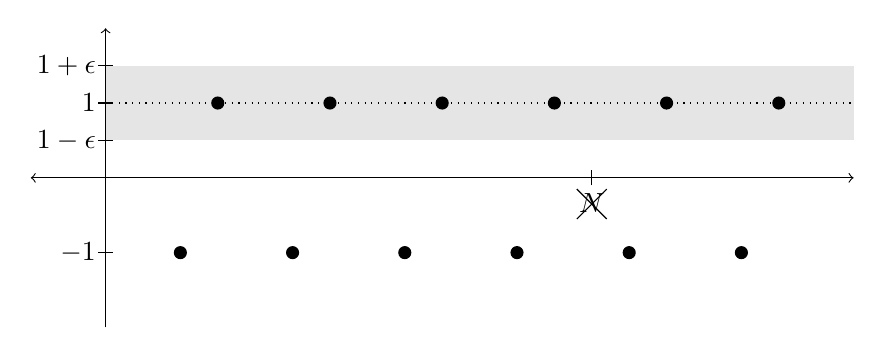
\begin{tikzpicture}[scale=0.95]
      % Shaded region, drawn first so it goes behind everything
      \fill[gray!20] (0,1-0.5) rectangle (10,1+0.5);

      % Axes
      \draw[->] (0,-2) -- (0,2);
      \draw[<->] (-1,0) -- (10,0);

      % Tick marks on y-axis with small lines
      \draw (-0.1,1.5) -- (0.1,1.5);  % 1+epsilon
      \draw (-0.1,1) -- (0.1,1);      % 1
      \draw (-0.1,0.5) -- (0.1,0.5);  % 1-epsilon
      \draw (-0.1,-1) -- (0.1,-1);    % -1

      % Labels
      \node[left] at (0,1) {$1$};
      \node[left] at (0,-1) {$-1$};
      \node[left] at (0,1.5) {$1+\epsilon$};
      \node[left] at (0,0.5) {$1-\epsilon$};

      % Dotted line at y=1
      \draw[dotted] (0,1) -- (10,1);

      % Points at y=1
      \foreach \x in {1.5, 3, 4.5, 6, 7.5, 9} {
        \filldraw (\x,1) circle (0.08);
      }

      % Points at y=-1
      \foreach \x in {1, 2.5, 4, 5.5, 7, 8.5} {
        \filldraw (\x,-1) circle (0.08);
      }

      % N marker with proper cross (X)
      \node[below, yshift=-2pt] at (6.5,0) {$N$};
      \draw (6.3,-0.55) -- (6.7,-0.15);
      \draw (6.3,-0.15) -- (6.7,-0.55);

      % Tick mark for N on x-axis
      \draw (6.5,-0.1) -- (6.5,0.1);
    \end{tikzpicture}
  \end{tightfigure}
  It likewise can't converge to $-1$. One might guess $0$, since that
  is halfway between $-1$ and $1$, but that also doesn't make sense
  since $a_n$ is always a distance of $1$ away from $0$, so it's
  certainly not getting ``closer and closer'' to $0$. (Or, $\epsilon
  = 1/2$ works again.) Ok, so we believe that it doesn't converge to
  anything, and we will use \outref{how-to-show-sequence-diverges} to show it.

  \begin{proof}
    Assume for a contradiction that there is
    some $a$ for which $a_n \to a$.
    Let $\epsilon = \frac{1}{2}$. Since we assumed that $a_n \to a$,
    there must be some $N$ for which, for all $n > N$, we have
    $\abs{a_n - a} < \frac{1}{2}$. That is, $\abs{(-1)^n - a} <
    \frac{1}{2}$ for all $n > N$. We proceed by cases.

    \underline{Even $n$.} If $n$ is even and $n > N$, then we have that
    \[ \abs{1 - a} < \frac{1}{2}. \]
    Unwinding this:
    \begin{gather*}
      -\frac{1}{2} < 1 - a < \frac{1}{2} \\
      -\frac{3}{2} < -a < -\frac{1}{2} \\
      \frac{1}{2} < a < \frac{3}{2}.
    \end{gather*}

    \underline{Odd $n$.} If $n$ is odd and $n > N$, then we have that
    \[ \abs{-1 - a} < \frac{1}{2}. \]
    Unwinding this:
    \begin{gather*}
      -\frac{1}{2} < -1 - a < \frac{1}{2} \\
      \frac{1}{2} < -a < \frac{3}{2} \\
      -\frac{3}{2} < a < -\frac{1}{2}.
    \end{gather*}

    But this is a contradiction; clearly no $a$ can be inside of both
    $\left(\frac{1}{2}, \frac{3}{2}\right)$ and $\left(-\frac{3}{2},
    -\frac{1}{2}\right)$.
    And so we must have $a_n \not\to a$.
  \end{proof}

  Essentially, focusing on the even case created a ball around $1$,
  of radius $\frac{1}{2}$, which $a_n$ would have to live within
  for all $n > N$.
  The odd case created a ball around $-1$, of radius $\frac{1}{2}$,
  which $a_n$ would have to live within for all $n > N$.
  But these two balls are disjoint, so $a_n$ can't live in both,
  creating a contradiction.

  \begin{tightfigure}
    \centering
    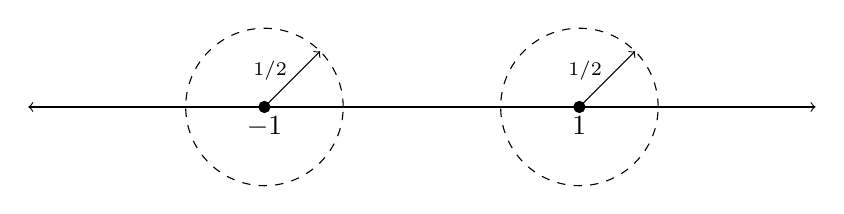
\begin{tikzpicture}
      % Draw the number line
      \draw[<->] (-5, 0) -- (5, 0);

      % Draw the points -1 and 1
      \filldraw (-2, 0) circle (2pt) node[below] {$-1$};
      \filldraw (2, 0) circle (2pt) node[below] {$1$};

      % Draw the circles around -1 and 1
      \draw[dashed] (-2, 0) circle (1);
      \draw[dashed] (2, 0) circle (1);

      % Add arrows from the center to the perimeter at 45 degrees
      \draw[->] (-2, 0) -- ++(45:1) node[midway, above,
      font=\scriptsize, xshift=-8pt, yshift=-4pt] {$1/2$};
      \draw[->] (2, 0) -- ++(45:1) node[midway, above,
      font=\scriptsize, xshift=-8pt, yshift=-4pt] {$1/2$};
    \end{tikzpicture}
  \end{tightfigure}

  Now here's another proof using the triangle inequality
  (\thmref{triangle-inequality}).

  \begin{proof}
    Again, let $\epsilon = \frac{1}{2}$. The even case still gives
    $\abs{1 - a} < \frac{1}{2}$, and the odd case still gives
    $\abs{-1 - a} < \frac{1}{2}$; although in the odd case we will
    rewrite $\abs{-1 - a}$ as $\abs{1 + a}$. Then, by the triangle inequality:
    \[ 2 = \abs{(1 - a) + (1 + a)} \leq \abs{1 - a} + \abs{1 + a}. \]
    But each of the absolute values on the right are assumed to be
    less than $\frac{1}{2}$. So,
    \[ 2 = \abs{(1 - a) + (1 + a)} \leq \abs{1 - a} + \abs{1 + a} <
    \frac{1}{2} + \frac{1}{2} = 1. \]
    So $2 < 1$? Preposterous! We have our contradiction.
  \end{proof}
\end{example}

\begin{proposition}[Limits are unique]
  A sequence cannot have more than one limit.
\end{proposition}

\begin{proofidea}
  The idea is to assume that you have a sequence $a$, that converges
  to some $a$ and also converges to some other number 6. Since it
  converges to $a$, after some point all the sequence points are
  within $\epsilon$ of $a$, for some really tiny $\epsilon$. But
  since it also converges to $b$, the same thing must happen there
  too. So if $\epsilon$ is small enough that those two regions are
  mutually exclusive, we will have a contradiction.

  \begin{tightfigure}
    \centering
    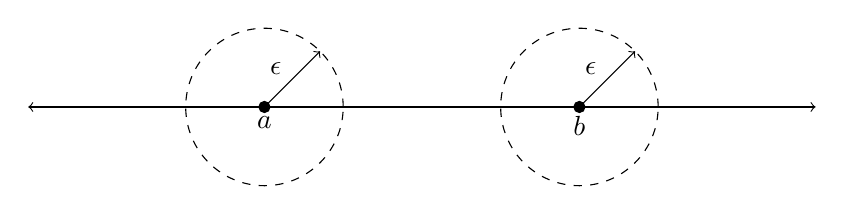
\begin{tikzpicture}
      % Draw the number line
      \draw[<->] (-5, 0) -- (5, 0);

      % Draw the points -1 and 1
      \filldraw (-2, 0) circle (2pt) node[below] {$a$};
      \filldraw (2, 0) circle (2pt) node[below] {$b$};

      % Draw the circles around -1 and 1
      \draw[dashed] (-2, 0) circle (1);
      \draw[dashed] (2, 0) circle (1);

      % Add arrows from the center to the perimeter at 45 degrees
      \draw[->] (-2, 0) -- ++(45:1) node[midway, above,
      xshift=-6pt, yshift=-2pt] {$\epsilon$};
      \draw[->] (2, 0) -- ++(45:1) node[midway, above,
      xshift=-6pt, yshift=-2pt] {$\epsilon$};
    \end{tikzpicture}
  \end{tightfigure}

  And this is how we will reach a contradiction: there is no way for
  $a_n (n > N)$ to be in both circles at the same time. Of course, if
  a and b are really close together we will need to choose a smaller
  $\epsilon$ to make sure the intervals remain disjoint, but that's
  the only difference.

  \begin{tightfigure}
    \centering
    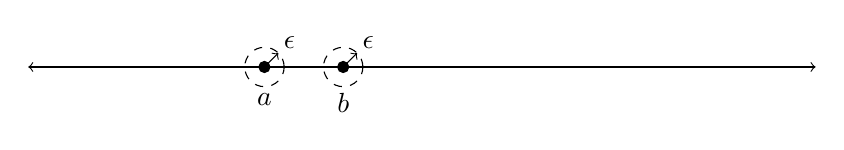
\begin{tikzpicture}
      % Draw the number line
      \draw[<->] (-5, 0) -- (5, 0);

      % Draw the points -1 and 1
      \filldraw (-2, 0) circle (2pt) node[below, yshift=-6pt] {$a$};
      \filldraw (-1, 0) circle (2pt) node[below, yshift=-6pt] {$b$};

      % Draw the circles around -1 and 1
      \draw[dashed] (-2, 0) circle (0.25);
      \draw[dashed] (-1, 0) circle (0.25);

      % Add arrows from the center to the perimeter at 45 degrees
      \draw[->] (-2, 0) -- ++(45:0.25) node[above, xshift=4pt,
      yshift=-2pt] {$\epsilon$};
      \draw[->] (-1, 0) -- ++(45:0.25) node[above, xshift=4pt,
      yshift=-2pt] {$\epsilon$};
    \end{tikzpicture}
  \end{tightfigure}

  For instance, if the radius of those balls is a third of the
  distance between $a$ and $b$, it should work out. With that
  intuition in mind, here's the proof.
\end{proofidea}

\begin{proof}
  Suppose for a contradiction that $a_n \to a$ and $a_n \to b$, where
  $a \neq b$; moreover, without loss of generality let's assume $a <
  b$. Let $\epsilon = (b - a)/3 > 0$. Since $a_n \to a$ there
  exists some $N_1$ such that for $n > N_1$ we have $|a_n - a| < (b -
  a)/3$. Likewise, since $a_n \to b$ there exists some $N_2$ such
  that for $n > N_2$ we have $|a_n - b| < (b - a)/3$. Let $N =
  \max\{N_1, N_2\}$. Then for $n > N$ (implying $n > N_1$ and $n >
  N_2$), we have both $|a_n - a| < (b - a)/3$ and $|a_n - b| < (b -
  a)/3$. That is, for such $n$ we have
  \[ -\frac{b-a}{3} < a_n - a < \frac{b-a}{3} \qquad \text{and}
  \qquad -\frac{b-a}{3} < a_n - b < \frac{b-a}{3}. \]
  i.e.,
  \[ a - \frac{b-a}{3} < a_n < a + \frac{b-a}{3} \qquad \text{and}
  \qquad b - \frac{b-a}{3} < a_n < b + \frac{b-a}{3}. \]
  In particular,
  \[ a_n < \frac{b+2a}{3} \qquad \text{and} \qquad \frac{2b+a}{3} < a_n. \]
  But since $a < b$, we must have $b + 2a < 2b + a$. But this then implies that
  \[ a_n < \frac{b+2a}{3} < \frac{2b+a}{3} < a_n, \]
  which is clearly a contradiction.
\end{proof}

There is a second proof that is even a little shorter.

\begin{proofidea}
  The idea is to show that $\abs{a - b} < \epsilon$ for all $\epsilon
  > 0$, and therefore $\abs{a - b} = 0$, implying that $a = b$.
  Intuitively, the way to show this is to say that if $a$, is getting
  really close to both $a$ and $b$, then that forces $a$ and $b$ to
  be close to each other. If we demand that $a_n$, is within
  $\epsilon/2$ of both $a$ and $b$, then the distance between $a$ and
  $b$ can't be more than $\epsilon$:

  \begin{tightfigure}
    \centering
    \begin{tikzpicture}
      % Draw the number line
      \draw[<->] (-5, 0) -- (5, 0);

      % Draw the points -1 and 1
      \filldraw (-2, 0) circle (2pt) node[below] {$a$};
      \filldraw (2, 0) circle (2pt) node[below] {$b$};

      % Draw the circles around -1 and 1
      \draw[dashed] (-2, 0) circle (2.25);
      \draw[dashed] (2, 0) circle (2.25);

      % Add arrows from the center to the perimeter at 45 degrees
      \draw[->] (-2, 0) -- ++(45:2.25) node[midway, above,
      xshift=-6pt, yshift=-2pt] {$\epsilon$};
      \draw[->] (2, 0) -- ++(45:2.25) node[midway, above,
      xshift=-6pt, yshift=-2pt] {$\epsilon$};
    \end{tikzpicture}
  \end{tightfigure}

  Using the triangle inequality we can then bound the distance from
  $a$ to $b$ by finding the distance from $a$ to $a_n$, plus the
  distance from $a_n$ to $b$.
\end{proofidea}

\begin{proof}
  Let $\epsilon > 0$. Since $\epsilon/2 > 0$ and $a_n \to a$,
  there exists some $N_1$ such that for $n > N_1$ we have $\abs{a_n -
  a} < \epsilon/2$. Since $\epsilon/2 > 0$ and $a_n \to b$,
  there exists some $N_2$ such that for $n > N_2$ we have $\abs{a_n -
  b} < \epsilon/2$. Let $N = \max(N_1, N_2)$ and pick any $n > N$. Then
  \begin{align*}
    \abs{a - b} &= \abs{a - a_n + a_n - b} \\
    &\leq \abs{a - a_n} + \abs{a_n - b} && \text{(triangle inequality)} \\
    &= \abs{a_n - a} + \abs{a_n - b} \\
    &< \epsilon/2 + \epsilon/2 && \text{($n > N$ implies $n >
    N_1$ and $n > N_2$)} \\
    &= \epsilon.
  \end{align*}
  Since this holds for any $\epsilon > 0$, we have shown that
  $\abs{a - b} < \epsilon$ for all $\epsilon > 0$, which
  implies that $\abs{a - b} = 0$, and hence $a = b$. So indeed, $a_n$
  can converge to only a single point.
\end{proof}

\begin{proposition}
  \prplabel{convergence-implies-bounded}
  If $(a_n)$ is a convergent sequence, then $(a_n)$ is bounded.
\end{proposition}

\begin{proof}
  Since $(a_n)$ is convergent, let $a$ be the value it is converging
  to. By the definition of convergence (with $\epsilon = 1$), there
  is some $N$ where
  \[ \abs{a_n - a} < 1 \]
  for all $n > N$. That is, $a - 1 < a_n < a + 1$ for all $n > N$. Let
  \[ U = \max \{a_1, a_2, a_3, \dots, a_N, a + 1\} \]
  and
  \[ L = \min \{a_1, a_2, a_3, \dots, a_N, a - 1\}. \]
  Note that if $n \leq N$, then $L \leq a_n \leq U$, since each such
  $a_n$ is included in the sets which we are taking the minimum and
  maximum of. And if $n > N$, then we already noted that $a - 1 < a_n
  < a + 1$, which implies that
  \[ L \leq a - 1 < a_n < a + 1 \leq U, \]
  and hence $L < a_n < U$. Combining these cases, we have that
  \[ L \leq a_n \leq U \]
  for all $n$. And thus, by definition, $(a_n)$ is bounded.
\end{proof}

\begin{corollary}
  If $(a_n)$ is an unbounded sequence, then $(a_n)$ is divergent.
\end{corollary}

\begin{theorem}[Sequence limit laws]
  \thmlabel{sequence-limit-laws}
  Assume that $(a_n)$ and $(b_n)$ are convergent sequences of real
  numbers such that $a_n \to a$ and $b_n \to b$. Also assume that $c
  \in \RR$. Then,
  \begin{enumerate}
    \item $(a_n + b_n) \to a + b$.
    \item $(a_n - b_n) \to a - b$.
    \item $(a_n \cdot b_n) \to a \cdot b$.
    \item $(\frac{a_n}{b_n}) \to \frac{a}{b}$, provided each $b \neq
      0$ and each $b_n \neq 0$.
    \item $(c \cdot a_n) \to c \cdot a$.
  \end{enumerate}
\end{theorem}

\begin{example}
  What is
  \[ \lim_{n\to\infty} \frac{1}{2} \cdot \left(\frac{\frac{1}{n} +
    \frac{1}{n^2} + 4}{5 - \frac{1}{n^2}}\right) \cdot
  \left(\frac{3n+1}{n+2} + \frac{1}{\sqrt{n}}\right)? \]
  By the limit laws, we have
  \begin{align*}
    \lim_{n\to\infty} \frac{1}{2} \cdot \left(\frac{\frac{1}{n} +
    \frac{1}{n^2} + 4}{5 - \frac{1}{n^2}}\right) \cdot
    \left(\frac{3n+1}{n+2} + \frac{1}{\sqrt{n}}\right) = \frac{1}{2}
    \cdot \left(\frac{0 + 0 + 4}{5}\right) \cdot (3 + 0) = \frac{6}{5}.
  \end{align*}
\end{example}

\begin{theorem}[Sequence squeeze theorem]
  \thmlabel{sequence-squeeze}
  Assume $a_n \leq x_n \leq b_n$ for all $n$. Furthermore, assume that
  \[ a_n \to L \qquad \text{and} \qquad b_n \to L. \]
  Then,
  \[ x_n \to L. \]
\end{theorem}

\begin{proof}
  Let $\epsilon > 0$.
  \begin{itemize}
    \item Since $a_n \to L$, there exists some $N_1$ such that $n >
      N_1$ implies $\abs{a_n - L} < \epsilon$. That is, $-\epsilon <
      a_n - L < \epsilon$. Or,
      \[ L - \epsilon < a_n < L + \epsilon. \tag{1} \]

    \item Since $b_n \to L$, there exists some $N_2$ such that $n >
      N_2$ implies $\abs{b_n - L} < \epsilon$. That is, $-\epsilon <
      b_n - L < \epsilon$. Or,
      \[ L - \epsilon < b_n < L + \epsilon. \tag{2} \]
  \end{itemize}

  Let $N = \max(N_1, N_2)$, and let $n > N$. Combining the
  inequality $a_n \leq x_n \leq b_n$ with the left half of (1) and
  the right half of (2), we get
  \begin{gather*}
    L - \epsilon < a_n \leq x_n \leq b_n < L + \epsilon \\
    L - \epsilon < x_n < L + \epsilon \\
    -\epsilon < x_n - L < \epsilon \\
    \abs{x_n - L} < \epsilon.
  \end{gather*}
  \vspace{-1em}
\end{proof}

\begin{example}
  Prove that
  \[ \lim_{n \to \infty} \frac{1}{n^{2.7} + \sqrt{n} + \pi} = 0. \]

  \begin{proof}
    Since
    \[ 0 \leq \frac{1}{n^{2.7} + \sqrt{n} + \pi} \leq \frac{1}{n},
      \qquad \lim_{n \to \infty} 0 = 0, \qquad \text{and} \qquad \lim_{n
    \to \infty} \frac{1}{n} = 0, \]
    by the sequence squeeze theorem (\thmref{sequence-squeeze}),
    \[ \lim_{n \to \infty} \frac{1}{n^{2.7} + \sqrt{n} + \pi} = 0. \]
  \end{proof}
\end{example}

\begin{definition}[Monotone sequences]
  A sequence $(a_n)$ is \vocab{monotone increasing} if $a_n \leq a_{n
  + 1}$ for all $n$. Likewise, a sequence $(a_n)$ is \vocab{monotone
  decreasing} if $a_n \geq a_{n + 1}$ for all $n$. If it is either
  monotone increasing or monotone decreasing, it is \vocab{monotone}.
\end{definition}

\begin{theorem}[The monotone convergence theorem]
  \thmlabel{monotone-convergence}
  Suppose $(a_n)$ is monotone. Then $(a_n)$ converges if and only if
  it is bounded. Moreover,
  \begin{itemize}
    \item If $(a_n)$ is increasing, then either $(a_n)$ diverges to
      $\infty$ or
      \[ \lim_{n \to \infty} a_n = \sup(\set{a_n : n \in \NN}). \]
    \item If $(a_n)$ is decreasing, then either $(a_n)$ diverges to
      $-\infty$ or
      \[ \lim_{n \to \infty} a_n = \inf(\set{a_n : n \in \NN}). \]
  \end{itemize}
\end{theorem}

\begin{proofidea}
  Suppose $(a_n)$ is monotonically increasing. If it's not bounded,
  then given any $M > 0$, this $M$ is not an upper bound and so
  eventually $(a_n)$ will get above it. And since it's monotonically
  increasing, once it gets above a number, it \textit{stays} above that number.

  \begin{tightfigure}
    \centering
    \begin{tikzpicture}[scale=0.75]
      % Draw the coordinate axes
      \draw[<->] (-2,0) -- (12,0);
      \draw[<->] (0,-1.5) -- (0,6);

      % Draw the horizontal line at M (solid, not dashed)
      \draw (-0.1,3.5) -- (0.1,3.5) node[left, xshift=-2pt] {$M$};

      % Plot the monotone sequence points following a y = 0.1x² curve
      \foreach \x/\y in {1/0.55, 2/0.7, 3/0.95, 4/1.3, 5/1.75,
      6/2.3, 7/2.95, 8/3.7, 9/4.55, 10/5.5}
      \filldraw[black] (\x,\y) circle (0.09);

      % Add the arrows pointing to points above M with proper angle
      \draw[->] (6,5.4) -- (9.1,5.5);
      \draw[->] (6,5) -- (8.2,4.65);
      \draw[->] (6,4.6) -- (7.4,4);

      % Add the text
      \node[align=center, font=\small] at (3.5,5) {Once a monotone
      \\ $(a_n)$ gets above $M$, \\ it stays above $M$.};
    \end{tikzpicture}
  \end{tightfigure}

  If, on the other hand, $(a_n)$ is bounded, then the sequence must
  be leveling out (it's monotone, so it can't go up and down).

  \begin{tightfigure}
    \centering
    \begin{tikzpicture}[scale=0.75]
      % Draw the coordinate axes
      \draw[<->] (-2,0) -- (12,0);
      \draw[<->] (0,-1.5) -- (0,6);

      % Draw the horizontal dashed line for the least upper bound
      \draw[dashed] (-0.1,4) -- (12,4);

      % Plot the monotone sequence points with diminishing increases
      % (approaching the bound)
      \filldraw[black] (1,0.9) circle (0.09);
      \filldraw[black] (2,1.8) circle (0.09);
      \filldraw[black] (3,2.4) circle (0.09);
      \filldraw[black] (4,2.9) circle (0.09);
      \filldraw[black] (5,3.2) circle (0.09);
      \filldraw[black] (6,3.4) circle (0.09);
      \filldraw[black] (7,3.6) circle (0.09);
      \filldraw[black] (8,3.7) circle (0.09);
      \filldraw[black] (9,3.8) circle (0.09);
      \filldraw[black] (10,3.85) circle (0.09);

      % Add the curved arrow pointing to the least upper bound
      \draw[->] (4.75,5.5) to[out=180, in=90] (3,4);

      % Add the text
      \node[align=center, font=\small] at (8,5.5) {$(a_n)$'s
      bounded above, so \\ there's a least upper bound};
    \end{tikzpicture}
    \vspace{-1.5em}
  \end{tightfigure}
\end{proofidea}

\begin{proof}
  Assume that $(a_n)$ is monotonically increasing, and let's suppose
  first that $a_n$ is not bounded. Then for any $M > 0$ there exists
  some $N$ such that $a_N > M$. But since $(a_N)$ is monotonically
  increasing, for $n > N$ we have a$_n \geq a_N > M$. And so, by
  \defref{divergent-sequences}, $(a_n)$ diverges to $\infty$.

  Next suppose that $(a_n)$ is bounded. Then we have that $\set{a_n :
  n \in \NN}$ is a subset of $\RR$ which is bounded above, which by
  the completeness of $\RR$ implies that $\sup(\set{a_n : n \in
  \NN})$ exists. Call this supremum $\alpha$. We want to show that
  $\lim_{n \to \infty} a_n = \alpha$; that is, we want to show that
  for any $\epsilon > 0$ there exists some $N$ such that $n > N$
  implies $\size{a_n — \alpha} < \epsilon$.

  To show this, first let $\epsilon > 0$. Since $\sup(\set{a_n : n
  \in \NN}) = \alpha$, by the analytic definition of suprema
  (\thmref{suprema-analytically}) there exists some $a_N > a -
  \epsilon$. And since $(a_n)$ is monotonically increasing, we see
  that for any $n > N$ we have that $a_n \geq a_N > \alpha -
  \epsilon$. And of course, $a_n < \alpha$ due to the fact that
  $\alpha$ is the supremum (and hence an upper bound) of $\set{a_n :
  n \in \NN}$. And so, for $n > N$, we have $\alpha - \epsilon < a_n
  < \alpha$. This implies $\alpha - \epsilon < a_n < \alpha +
  \epsilon$, and hence $-\epsilon < a_n - \alpha < \epsilon$, which,
  at last, gives
  \[ \size{a_n - \alpha} < \epsilon \]
  completing the proof in the case when $(a_n)$ is monotonically increasing.

  The case where $(a_n)$ is monotonically decreasing is very similar.
\end{proof}

\begin{remark}
  This theorem is nice for several reasons, but one of which is the
  fact that you do not have to know what the limit of $(a_n)$ is in
  order to show that $(a_n)$ is convergent. This is notable since in
  the definition of sequence convergence---which, until now, we have
  heavily relied on to show a sequence converges---requires that you
  already know (and can write down) what the limit is going to be.
  Below is an example where it would be quite a challenge to write
  down the limit of the sequence in a beneficial way. Yet by the
  monotone convergence theorem, we will be able to conclude that the
  limit exists.
\end{remark}

\begin{example}
  Let $(a_n)$ be the sequence where $a_1 = 0.1$, $a_2 = 0.12$, $a_3 =
  0.123$, $a_4 = 0.1234$, and so on. (And, to be clear, this pattern
    does not change when you reach double digits. For example, $a_{12}
  = 0.123456789101112$.) Prove that $(a_n)$ converges.

  \begin{proof}
    Note that $a_{n+1}$ and $a_n$ match exactly until the last digits
    of $a_{n+1}$, which are the digits of $n + 1$. Therefore,
    $a_{n+1} - a_n$ is a number with a bunch of zeros followed the
    digits of $n + 1$. In particular,
    \[ a_{n+1} - a_n > 0 \]
    for all $n$. We have shown that $a_{n+1} > a_n$ for all $n$,
    proving that $(a_n)$ is monotone increasing. Furthermore note
    that since all the terms begin with $0.1$, we have that $a_n \leq
    1$ for all $n$.

    We have shown that $(a_n)$ is monotone increasing and bounded
    above, therefore by the monotone convergence theorem
    (\thmref{monotone-convergence}) the sequence converges,
    completing the proof.
  \end{proof}
\end{example}

\begin{proposition}
  Suppose $S \subseteq \RR$ is bounded above. Then there exists a
  sequence $(a_n)$ where $a_n \in S$ for each $n$ and
  \[ \lim_{n \to \infty} a_n = \sup(S). \]
  Likewise, if $S$ is bounded below, then there exists a sequence
  $(b_n)$ where $b_n \in S$ for each $n$ and
  \[ \lim_{n \to \infty} b_n = \inf(S). \]
\end{proposition}

\begin{proofidea}
  We need to find elements of $S$ which are getting closer and closer
  to $\sup(S)$.
  What was our \textit{super} useful theorem for doing just that? The
  analytic definition of suprema (\thmref{suprema-analytically})!
  That was the theorem that said for any $\epsilon > 0$, there exists
  some $a \in S$ such that $a > \sup(S) - \epsilon$.
  And since it works for any $\epsilon > 0$, we can choose a sequence
  of $\epsilon$ values that are getting closer and closer to $0$,
  which in turn produce a sequence of $a$ values that are getting
  closer and closer to $\sup(S)$.

  And once we have found a sequence of these elements which are
  getting closer and closer to $\sup(S)$,
  how do we formally show they converge to $\sup(S)$? The sequence
  squeeze theorem (\thmref{sequence-squeeze})
  sure sounds like it's up to the job.
\end{proofidea}

\begin{proof}
  Suppose $S \subseteq \RR$ is bounded above, implying that $\sup(S)$
  exists. Let $\sup(S) = \alpha$ (implying $a_n \leq \alpha$ for all
  $n$). By the analytic definition of suprema
  (\thmref{suprema-analytically}), for any
  $\epsilon > 0$ there exists some $x \in S$ such that $x > \alpha -
  \epsilon$. In particular, there exists some $a_1 \in S$ such that
  $a_1 > \alpha - 1$; and there exists some $a_2 \in S$ such that
  $a_2 > \alpha - \frac{1}{2}$; and there exists some $a_3 \in S$
  such that $a_3 > \alpha - \frac{1}{3}$; and, in general, for each
  $n \in \NN$ there exists some $a_n \in S$ such that $a_n > \alpha -
  \frac{1}{n}$.

  Thus we obtain a sequence $(a_n)$ from $S$. Moreover, this sequence
  does indeed converge to $\alpha$. Therefore, by
  the limit laws (\thmref{sequence-limit-laws}) we have that
  \[ \alpha - \frac{1}{n} \to \alpha - 0 = \alpha. \]
  So we have an inequality
  \[ \alpha - \frac{1}{n} \leq a_n \leq \alpha, \]
  where both the upper and lower bounds converge to $\alpha$. By the
  sequence squeeze theorem (\thmref{sequence-squeeze}) we see that $\lim_{n \to
  \infty} a_n = \alpha$, as desired.

  The infimum case is \textit{very} similar.
\end{proof}

\begin{definition}
  Let $(a_n)$ be a sequence of real numbers and let
  \[ n_1 < n_2 < n_3 < \dots \]
  be an increasing sequence of integers. Then,
  \[ a_{n_1}, a_{n_2}, a_{n_3}, \dots \]
  is called a \vocab{subsequence} of $(a_n)$, and is denoted $(a_{n_k})$.
\end{definition}

\begin{proposition}
  \prplabel{sequence-converges-iff-all-subsequences-converge}
  A sequence $(a_n)$ converges to $a$ if and only if every
  subsequence of $(a_n)$ also converges to $a$.
\end{proposition}

\begin{proof}
  \phantom{.}

  $(\Rightarrow)$ Assume that $(a_n)$ converges to $a$ and $(a_{n_k})$ is a
  subsequence of $(a_n)$. Let $\epsilon > 0$. Then there exists some
  $N$ such that
  \[ \abs{a_n - a} < \epsilon \tag{1} \]
  for all $n > N$.

  We want to show that $a_{n_k} \to a$. That is, we want to show that
  there exists some $N_1$ such that $\abs{a_{n_k} - a} < \epsilon$ for
  all $k > N_1$. Notice that since each $n_i \in \NN$ and
  \[ n_1 < n_2 < n_3 < \dots, \]
  that we have $n_k \geq k$. Therefore by letting $N_1 = N$, for any
  $k > N_1$ we then know that $n_k > N$, so by $(1)$ we have
  \[ \abs{a_{n_k} - a} < \epsilon. \]

  $(\Leftarrow)$ Assume that every subsequence of $(a_n)$ converges
  to $a$. Suppose, for contradiction, that $(a_n)$ does not converge
  to $a$. By \outref{how-to-show-sequence-diverges}, this means that
  there exists some
  $\epsilon_0 > 0$ such that for every $N \in \NN$, there is some $n > N$ with
  $\abs{a_n - a} \geq \epsilon_0$. Using this fact, we can
  inductively construct a subsequence of
  $(a_n)$ as follows:
  \begin{enumerate}
    \item Let $n_1$ be a natural number with $\abs{a_{n_1} - a} \geq
      \epsilon_0$.
    \item Having chosen $n_1, \dots, n_k$, let $n_{k+1} > n_k$
      be a natural number with $\abs{a_{n_{k+1}} - a} \geq \epsilon_0$.
  \end{enumerate}

  This process yields a subsequence $(a_{n_k})$ with the property that
  $\abs{a_{n_k} - a} \geq \epsilon_0$ for all $k \in \NN$. But this
  means that $(a_{n_k})$ cannot converge to $a$, which contradicts
  our assumption that every subsequence of $(a_n)$ converges to $a$.
  Therefore, $(a_n)$ must converge to $a$.
\end{proof}

\begin{corollary}
  If $(a_n)$ has a pair of subsequences converging to different
  limits, then $(a_n)$ diverges.
\end{corollary}

\begin{proof}
  Assume for a contradiction that $(a_n)$ converges. Say, $a_n \to
  L$. By \prpref{sequence-converges-iff-all-subsequences-converge},
  this implies that every subsequence also converges to $L$. This
  contradicts the
  assumption that there are subsequences converging to different limits.
\end{proof}

\begin{proposition}
  If a monotone sequence $(a_n)$ has a convergent subsequence, then
  $(a_n)$ converges too, and has the same limit.
\end{proposition}

\begin{proofidea}
  First recall that by
  \prpref{sequence-converges-iff-all-subsequences-converge}, a
  convergent sequence always has the same limit as any of its
  subsequences. So by this, our task reduces to showing that $(a_n)$ converges.

  A monotone sequence is convergent if and only if it is bounded (by
  the monotone convergence theorem). We are told that $(a_n)$ is
  monotone and to show that it's bounded, we use the assumption that
  it has a convergent subsequence, $(a_{n_k})$. Here's the
  progression: $(a_n)$ being monotone implies that its subsequence is
  too, and $(a_{n_k})$ being convergent (and now monotone) will mean
  that $(a_n)$ is bounded too.
\end{proofidea}

\begin{proof}
  Assume that $(a_n)$ is monotone increasing; the case where $(a_n)$
  is monotone decreasing is \textit{very} similar.

  Let $(a_{n_k})$ be a convergent subsequence of $(a_n)$ and observe
  that since $(a_n)$ is monotone increasing, being a subsequence
  means that $(a_{n_k})$'s terms come from $(a_n)$ and do so in the
  same order as they appear in $(a_n)$, implying that $(a_{n_k})$ is
  also monotone increasing. That is, $(a_{n_k})$ was assumed to be
  convergent and was shown to be monotone---by the monotone
  convergence theorem (\thmref{monotone-convergence}) this means
  $(a_{n_k})$ converges, and in particular converges to
  $\sup(\{a_{n_k} : k \in \NN\})$.

  We now show that $(a_n)$ is convergent, again by using the monotone
  convergence theorem. Since $(a_n)$ is monotone increasing by
  assumption, we need only show that $(a_n)$ is bounded above. To see
  this, observe that since the subsequence $(a_{n_k})$ is an infinite
  list of elements from $(a_n)$, any particular element $a_n$ from
  the sequence has an element $a_{n_k}$ from this subsequence that
  comes after it. And since both $a_n$ and $a_{n_k}$ are terms of
  $(a_n)$, which is monotone increasing, we have $a_n \leq a_{n_k}$. So we have
  \[ a_n \leq a_{n_k} \leq \sup(\{a_{n_k} : k \in \NN\}), \]
  which proves that $(a_n)$ is bounded above (by this supremum), and
  so by the monotone convergence theorem we have proven that $(a_n)$ converges.

  Finally, since we have shown that the sequence $(a_n)$ is
  convergent, by Proposition 3.32 it has the same limit as any of its
  subsequences. This means that $(a_n)$ must also be converging to
  $\sup(\{a_{n_k} : k \in \NN\})$, completing the proof.
\end{proof}

\begin{lemma}
  \lemlabel{every-sequence-has-monotone-subsequence}
  Every sequence has a monotone subsequence.
\end{lemma}

\begin{proofidea}
  Here's the idea behind it. We draw a sequence of in the $xy$-plane
  by just plotting the points, and we will connect the dots to make a
  zig-zagged line:

  \begin{tightfigure}
    \centering
    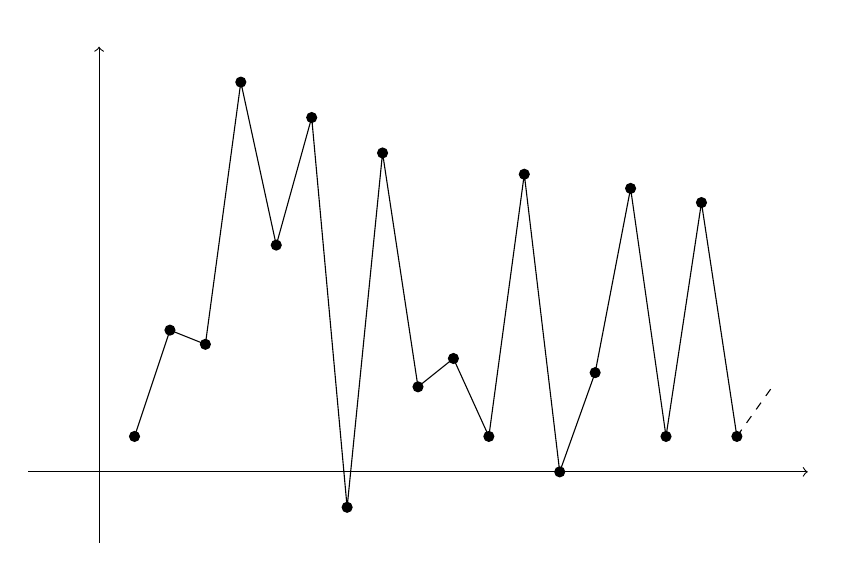
\begin{tikzpicture}[scale=0.9]
      % Draw axes
      \draw[->] (-1,0) -- (10,0) node[right] {};
      \draw[->] (0,-1) -- (0,6) node[above] {};

      % Plot the points and connect them
      \draw
      (0.5,0.5) --
      (1,2) --
      (1.5,1.8) --
      (2,5.5) --
      (2.5,3.2) --
      (3,5) --
      (3.5,-0.5) --
      (4,4.5) --
      (4.5,1.2) --
      (5,1.6) --
      (5.5,0.5) --
      (6,4.2) --
      (6.5,0) --
      (7,1.4) --
      (7.5,4) --
      (8,0.5) --
      (8.5,3.8) --
      (9,0.5);

      \draw[dashed] (9,0.5) -- (9.5,1.2);

      % Add points at each vertex
      \filldraw (0.5,0.5) circle (2pt);
      \filldraw (1,2) circle (2pt);
      \filldraw (1.5,1.8) circle (2pt);
      \filldraw (2,5.5) circle (2pt);
      \filldraw (2.5,3.2) circle (2pt);
      \filldraw (3,5) circle (2pt);
      \filldraw (3.5,-0.5) circle (2pt);
      \filldraw (4,4.5) circle (2pt);
      \filldraw (4.5,1.2) circle (2pt);
      \filldraw (5,1.6) circle (2pt);
      \filldraw (5.5,0.5) circle (2pt);
      \filldraw (6,4.2) circle (2pt);
      \filldraw (6.5,0) circle (2pt);
      \filldraw (7,1.4) circle (2pt);
      \filldraw (7.5,4) circle (2pt);
      \filldraw (8,0.5) circle (2pt);
      \filldraw (8.5,3.8) circle (2pt);
      \filldraw (9,0.5) circle (2pt);
    \end{tikzpicture}
  \end{tightfigure}

  From this you can maybe spot a nice \textit{decreasing} sequence,
  which is of course monotone:

  \begin{tightfigure}
    \centering
    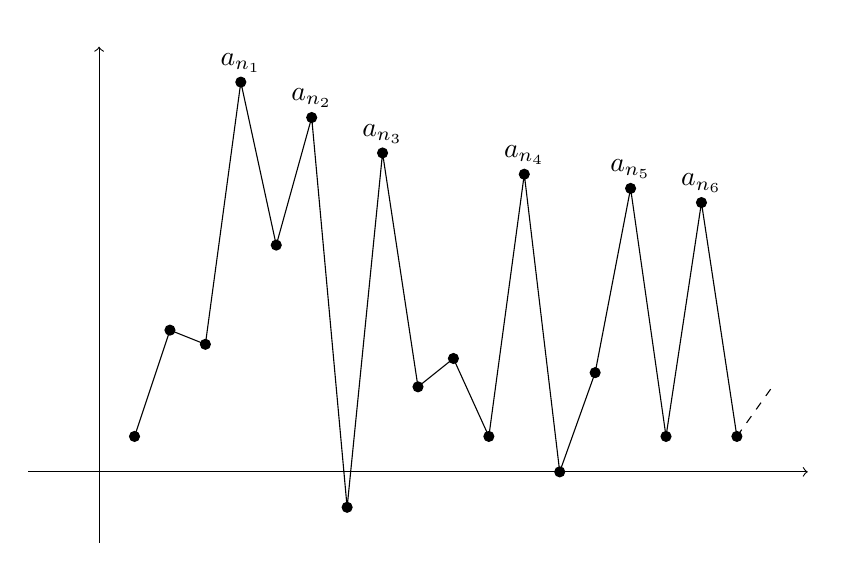
\begin{tikzpicture}[scale=0.9]
      % Draw axes
      \draw[->] (-1,0) -- (10,0) node[right] {};
      \draw[->] (0,-1) -- (0,6) node[above] {};

      % Plot the points and connect them
      \draw
      (0.5,0.5) --
      (1,2) --
      (1.5,1.8) --
      (2,5.5) --
      (2.5,3.2) --
      (3,5) --
      (3.5,-0.5) --
      (4,4.5) --
      (4.5,1.2) --
      (5,1.6) --
      (5.5,0.5) --
      (6,4.2) --
      (6.5,0) --
      (7,1.4) --
      (7.5,4) --
      (8,0.5) --
      (8.5,3.8) --
      (9,0.5);

      \draw[dashed] (9,0.5) -- (9.5,1.2);

      \filldraw (0.5,0.5) circle (2pt);
      \filldraw (1,2) circle (2pt);
      \filldraw (1.5,1.8) circle (2pt);
      \filldraw (2,5.5) circle (2pt) node[above] {$a_{n_1}$};
      \filldraw (2.5,3.2) circle (2pt);
      \filldraw (3,5) circle (2pt) node[above] {$a_{n_2}$};
      \filldraw (3.5,-0.5) circle (2pt);
      \filldraw (4,4.5) circle (2pt) node[above] {$a_{n_3}$};
      \filldraw (4.5,1.2) circle (2pt);
      \filldraw (5,1.6) circle (2pt);
      \filldraw (5.5,0.5) circle (2pt);
      \filldraw (6,4.2) circle (2pt) node[above] {$a_{n_4}$};
      \filldraw (6.5,0) circle (2pt);
      \filldraw (7,1.4) circle (2pt);
      \filldraw (7.5,4) circle (2pt) node[above] {$a_{n_5}$};
      \filldraw (8,0.5) circle (2pt);
      \filldraw (8.5,3.8) circle (2pt) node[above] {$a_{n_6}$};
      \filldraw (9,0.5) circle (2pt);
    \end{tikzpicture}
  \end{tightfigure}

  The magical definition that will solve everything is that of a
  \textit{peak}; we want those labeled points to form \textit{peaks},
  and we want to be able to say that if we have a(n infinite)
  sequence of peaks, then we do indeed have a decreasing sequence.
  The definition that does this is this: define a \textit{peak} to be
  a point $a_n$ which is larger than every later point; that is,
  $a_n$ is a peak if $a_n \geq a_m$ for all $m > n$.

  So if we have infinitely many peaks, then we obtain a sequence like
  the one above which will be decreasing. So what if we don't? Then
  we only have finitely many peaks. In this case, we can find an
  \textit{increasing} sequence, which is again monotone. To see how,
  just note that if you're past the last peak, then any point you
  pick is not a peak, which means there is some point after it which
  is larger. So one at a time you can pick larger and larger points,
  giving an increasing sequence.

  \begin{tightfigure}
    \centering
    \begin{tikzpicture}[scale=0.9]
      % Draw axes
      \draw[->] (-1,0) -- (10,0) node[right] {};
      \draw[->] (0,-1) -- (0,6) node[above] {};

      % Plot the points and connect them
      \draw
      (0.5,0.5) --
      (1,2) --
      (1.5,1.8) --
      (2,5.5) --
      (2.5,3.2) --
      (3,5) --
      (3.5,-0.5) --
      (4,0.5) --
      (4.5,-0.5) --
      (5,1) --
      (5.5,0) --
      (6,1.2) --
      (6.5,0.4) --
      (7,0) --
      (7.5,0.2) --
      (8,2) --
      (8.5,1.4) --
      (9,2.8);

      \draw[dashed] (9,2.8) -- (9.5,2.4);

      % Add points at each vertex
      \filldraw (0.5,0.5) circle (2pt);
      \filldraw (1,2) circle (2pt);
      \filldraw (1.5,1.8) circle (2pt);
      \filldraw (2,5.5) circle (2pt);
      \filldraw (2.5,3.2) circle (2pt);
      \filldraw (3,5) circle (2pt);
      \filldraw (3.5,-0.5) circle (2pt) node[below] {$a_{n_1}$};
      \filldraw (4,0.5) circle (2pt) node[above] {$a_{n_2}$};
      \filldraw (4.5,-0.5) circle (2pt);
      \filldraw (5,1) circle (2pt) node[above] {$a_{n_3}$};
      \filldraw (5.5,0) circle (2pt);
      \filldraw (6,1.2) circle (2pt) node[above] {$a_{n_4}$};
      \filldraw (6.5,0.4) circle (2pt);
      \filldraw (7,0) circle (2pt);
      \filldraw (7.5,0.2) circle (2pt);
      \filldraw (8,2) circle (2pt) node[above] {$a_{n_5}$};
      \filldraw (8.5,1.4) circle (2pt);
      \filldraw (9,2.8) circle (2pt) node[above] {$a_{n_6}$};
    \end{tikzpicture}
  \end{tightfigure}
\end{proofidea}

\begin{proof}
  Call $a_n$ a \textit{peak} if $a_n$ is larger than every later
  point. That is, if $a_n \geq a_m$ for all $m > n$.

  Either there are infinitely many peaks or finitely many peaks.
  Assume first that $(a_n)$ has infinitely many peaks. Then let
  $a_{n_k}$ be the $k$th peak. Then, by the definition of a peak,
  $a_{n_k} \geq a_{n_{k+1}}$, implying that $(a_{n_k})$ is a
  decreasing subsequence.

  Now assume that $(a_n)$ has finitely many peaks, and let $a_N$ be
  the last one. Then let $a_{n_1} = a_{N+1}$. Since $a_N$ was the
  last peak, $a_{N+1}$ is \textit{not} a
  peak, implying that there is some later point $a_{n_2}$ that is
  larger than it. Likewise, since $a_{n_2}$ is after the last peak,
  it is also not a peak, and so there must be some later point
  $a_{n_3}$ that is larger than it. Continuing in this way we
  construct an increasing subsequence $(a_{n_k})$.

  In either case we found a monotone subsequence, so we are done.
\end{proof}

\begin{theorem}[The Bolzano-Weierstrass theorem]
  \thmlabel{bolzano-weierstrass}
  Every bounded sequence has a convergent subsequence.
\end{theorem}

\begin{proof}
  Assume $(a_n)$ is a bounded sequence. Then by
  \lemref{every-sequence-has-monotone-subsequence} it has a monotone
  subsequence, $(a_{n_k})$. Also, since $(a_n)$ is bounded, so is
  $(a_{n_k})$. Since $(a_{n_k})$ is both bounded and monotone, by the
  monotone convergence theorem it converges.
\end{proof}

\begin{definition}
  A sequence $(a_n)$ is \vocab{Cauchy} if for all $\epsilon > 0$
  there exists some $N \in \NN$ such that
  \[ \abs{a_m - a_n} < \epsilon \]
  for all $m, n > N$.
\end{definition}

\begin{lemma}
  \lemlabel{cauchy-implies-bounded}
  If $(a_n)$ is Cauchy, then $(a_n)$ is bounded.
\end{lemma}

\begin{proof}
  Assume $(a_n)$ is Cauchy. Then (for $\epsilon = 1$) there exists
  some $N \in \NN$ such that
  \[ \abs{a_m - a_n} < 1 \]
  for all $m, n > N$. In particular, for all $n > N$,
  \[ \abs{a_n - a_{n+1}} < 1. \]
  Therefore for $n > N$, we know that the terms are bounded:
  \[ a_{N+1} - 1 < a_n < a_{N+1} + 1. \]
  And there are only finitely many points before $a_N$, so these are
  certainly bounded. Consequently, we can find a general bound on all
  $a_n$. Indeed, if we let
  \[ L = \min(\{a_1, a_2, a_3, \dots, a_N, a_{N+1} - 1\}) \]
  and
  \[ U = \max(\{a_1, a_2, a_3, \dots, a_N, a_{N+1} + 1\}), \]
  then
  \[ L \leq a_n \leq U \]
  for all $n \in \NN$. So $(a_n)$ is bounded.
\end{proof}

\begin{theorem}[Cauchy criterion for convergence]
  \thmlabel{cauchy-criterion-for-convergence}
  A sequence converges if and only if it is Cauchy.
\end{theorem}

\begin{proofsketch}
  For the forward direction, suppose $a_n$ converges to $a$. If $a_n$
  and $a_m$ are both within $\epsilon / 2$ of $a$, then they must be
  within $\epsilon$ of each other. We can formally show this using
  the triangle inequality.

  For the backwards direction, the idea is this: It will be helpful
  to identify what the Cauchy sequence is converging to. And by
  Bolzano-Weierstrass we can find a subsequence that is converging to
  some $a$. Our goal will then be to prove that $a$ is in fact the
  sequence's limit. How? Well, that subsequence gets super close to
  $a$. What about the terms in $(a_n)$ which are not in the
  subsequence? By the Cauchy criterion, they get super close to the
  elements of the subsequence! And if a term in the sequence is super
  close to a term of the subsequence, which is in turn super close to
  the limit... then the sequence must be close to the limit, too.
\end{proofsketch}

\begin{proof}
  \phantom{.}

  $(\Rightarrow)$ Assume that $(a_n)$ converges to some $a \in \RR$.
  Let $\epsilon > 0$. Since $\epsilon / 2 > 0$, there exists some $N
  \in \NN$ such that for any $n > N$ we have
  \[
    \abs{a_n - a} < \frac{\epsilon}{2}.
  \]
  Then, for any $n, m > N$,
  \[
    \abs{a_n - a_m} = \abs{a_n - a + a - a_m}
    \leq \abs{a_n - a} + \abs{a - a_m}
    < \frac{\epsilon}{2} + \frac{\epsilon}{2}
    = \epsilon.
  \]

  $(\Leftarrow)$ Assume that $(a_n)$ is Cauchy, and note that by
  \lemref{cauchy-implies-bounded}, $(a_n)$ is bounded.
  Combining these two facts, and applying the Bolzano-Weierstrass
  theorem (\thmref{bolzano-weierstrass}), we conclude that some
  subsequence of $(a_n)$ converges. Say, $(a_{n_j})$ converges to
  $a$. Our goal is to show that $(a_n)$ converges; we will in fact
  prove that $a_n \to a$.

  Let $\epsilon > 0$. Since $\epsilon / 2 > 0$ and $(a_n)$ is Cauchy,
  there exists some $N_1$ such that
  \[
    \abs{a_n - a_m} < \frac{\epsilon}{2} \tag{$1$}
  \]
  for all $n, m > N_1$. Since $\epsilon / 2 > 0$ and $(a_{n_j})$
  converges to $a$, there exists some $N_2$ such that $j > N_2$ implies
  \[
    \abs{a_{n_j} - a} < \frac{\epsilon}{2}. \tag{$2$}
  \]

  We want to choose some $J$ so that, for subscripts past this point,
  both $(1)$ and $(2)$ hold. Choose $J = \max(N_1,
  N_2)$. Notice, from the definition of a subsequence,
  that $n_j \geq j$. In particular, $n_{J+1} > J$. And so, for any $j > J$,
  \[
    \abs{a_j - a} = \abs{a_j - a_{n_{J+1}} + a_{n_{J+1}} - a}
    \leq \abs{a_j - a_{n_{J+1}}} + \abs{a_{n_{J+1}} - a}
    < \frac{\epsilon}{2} + \frac{\epsilon}{2}
    = \epsilon.
  \]
\end{proof}

\begin{theorem}[Stolz-Cesàro theorem]
  Let $(a_n)$ and $(b_n)$ be two sequences.
  \begin{enumerate}
    \item Assume that $a_n \to 0$ and $b_n \to 0$. Suppose $b_n$ is
      strictly decreasing and
      \[ \lim_{n \to \infty} \frac{a_{n + 1} - a_n}{b_{n + 1} - b_n} = a, \]
      where $a$ is finite or $+\infty$, then
      \[ \lim_{n \to \infty} \frac{a_n}{b_n} = \lim_{n \to \infty}
      \frac{a_{n + 1} - a_n}{b_{n + 1} - b_n} = a. \]
    \item Assume that $b_n$ is a strictly monotone and divergent
      sequence, i.e. strictly increasing and approaching $+\infty$,
      or strictly decreasing and approaching $-\infty$. Suppose
      \[ \lim_{n \to \infty} \frac{a_{n + 1} - a_n}{b_{n + 1} - b_n} = a, \]
      where $a$ is finite or $+\infty$ if $b_n$ increases, or $a$ is finite
      or $-\infty$ if $b_n$ decreases. Then,
      \[ \lim_{n \to \infty} \frac{a_n}{b_n} = \lim_{n \to \infty}
      \frac{a_{n + 1} - a_n}{b_{n + 1} - b_n} = a. \]
  \end{enumerate}
\end{theorem}

\begin{remark}
  Stolz-Cesàro theorem provides a powerful tool to evaluate limits of
  sequences, and is
  viewed as a discrete form of L'Hôpital's rule.
\end{remark}
